% =============================================================================
%  AeroTraj-Ultra — hybrid training objective, hand-written TikZ.
%
%  LaTeX-native version of docs/figures/hybrid_loss.png.  The two terms inherited
%  from the binary-encoding lineage are highlighted: one supervises the ENCODING
%  (the bit logits) and one supervises the TASK (the decoded trajectory), which is
%  possible only because the decoder is differentiable.
%
%  Build:  pdflatex hybrid_loss_tikz.tex
% =============================================================================
\documentclass[border=6pt]{standalone}

\usepackage[T1]{fontenc}
\usepackage{lmodern}
\usepackage{amsmath,amssymb}
\usepackage{tikz}
\usetikzlibrary{positioning, arrows.meta, fit, backgrounds, calc}

\definecolor{roleLoss}{HTML}{FFF2CC}
\definecolor{roleLossEdge}{HTML}{D6B656}
\definecolor{roleAdded}{HTML}{FFE6CC}
\definecolor{roleAddedEdge}{HTML}{D79B00}
\definecolor{roleModel}{HTML}{E1D5E7}
\definecolor{roleModelEdge}{HTML}{9673A6}
\definecolor{roleTgt}{HTML}{D5E8D4}
\definecolor{roleTgtEdge}{HTML}{82B366}
\definecolor{roleSum}{HTML}{F8CECC}
\definecolor{roleSumEdge}{HTML}{B85450}

\tikzset{
  blk/.style   = {draw, rounded corners=2.5pt, line width=0.75pt, align=center,
                  inner sep=4.5pt, font=\small, minimum height=0.95cm},
  model/.style = {blk, fill=roleModel, draw=roleModelEdge, text width=4.2cm},
  tgt/.style   = {blk, fill=roleTgt, draw=roleTgtEdge, text width=4.2cm},
  inherited/.style = {blk, fill=roleLoss, draw=roleLossEdge, text width=5.9cm},
  added/.style = {blk, fill=roleAdded, draw=roleAddedEdge, text width=5.9cm},
  total/.style = {blk, fill=roleSum, draw=roleSumEdge, text width=8.4cm},
  ar/.style    = {-{Latex[length=2.1mm, width=1.5mm]}, draw=black!70,
                  line width=0.7pt},
  bus/.style   = {draw=black!35, line width=0.7pt},
  small/.style = {font=\scriptsize, text=black!70},
  label/.style = {font=\scriptsize, text=black!60, inner sep=1.5pt},
  head/.style  = {font=\small\bfseries, text=black!75},
}

\newcommand{\bitrow}[3]{%
  \begin{scope}[shift={#1}]
  \foreach \i in {0,...,\numexpr#2-1\relax}{%
    \pgfmathparse{int(mod(\i,3)==0 || mod(\i,5)==0)}%
    \ifnum\pgfmathresult=1\fill[black!80] (\i*#3,0) rectangle ++(#3*0.72,#3*0.72);\fi
    \draw[black!55, line width=0.25pt] (\i*#3,0) rectangle ++(#3*0.72,#3*0.72);%
  }%
  \end{scope}%
}

\begin{document}
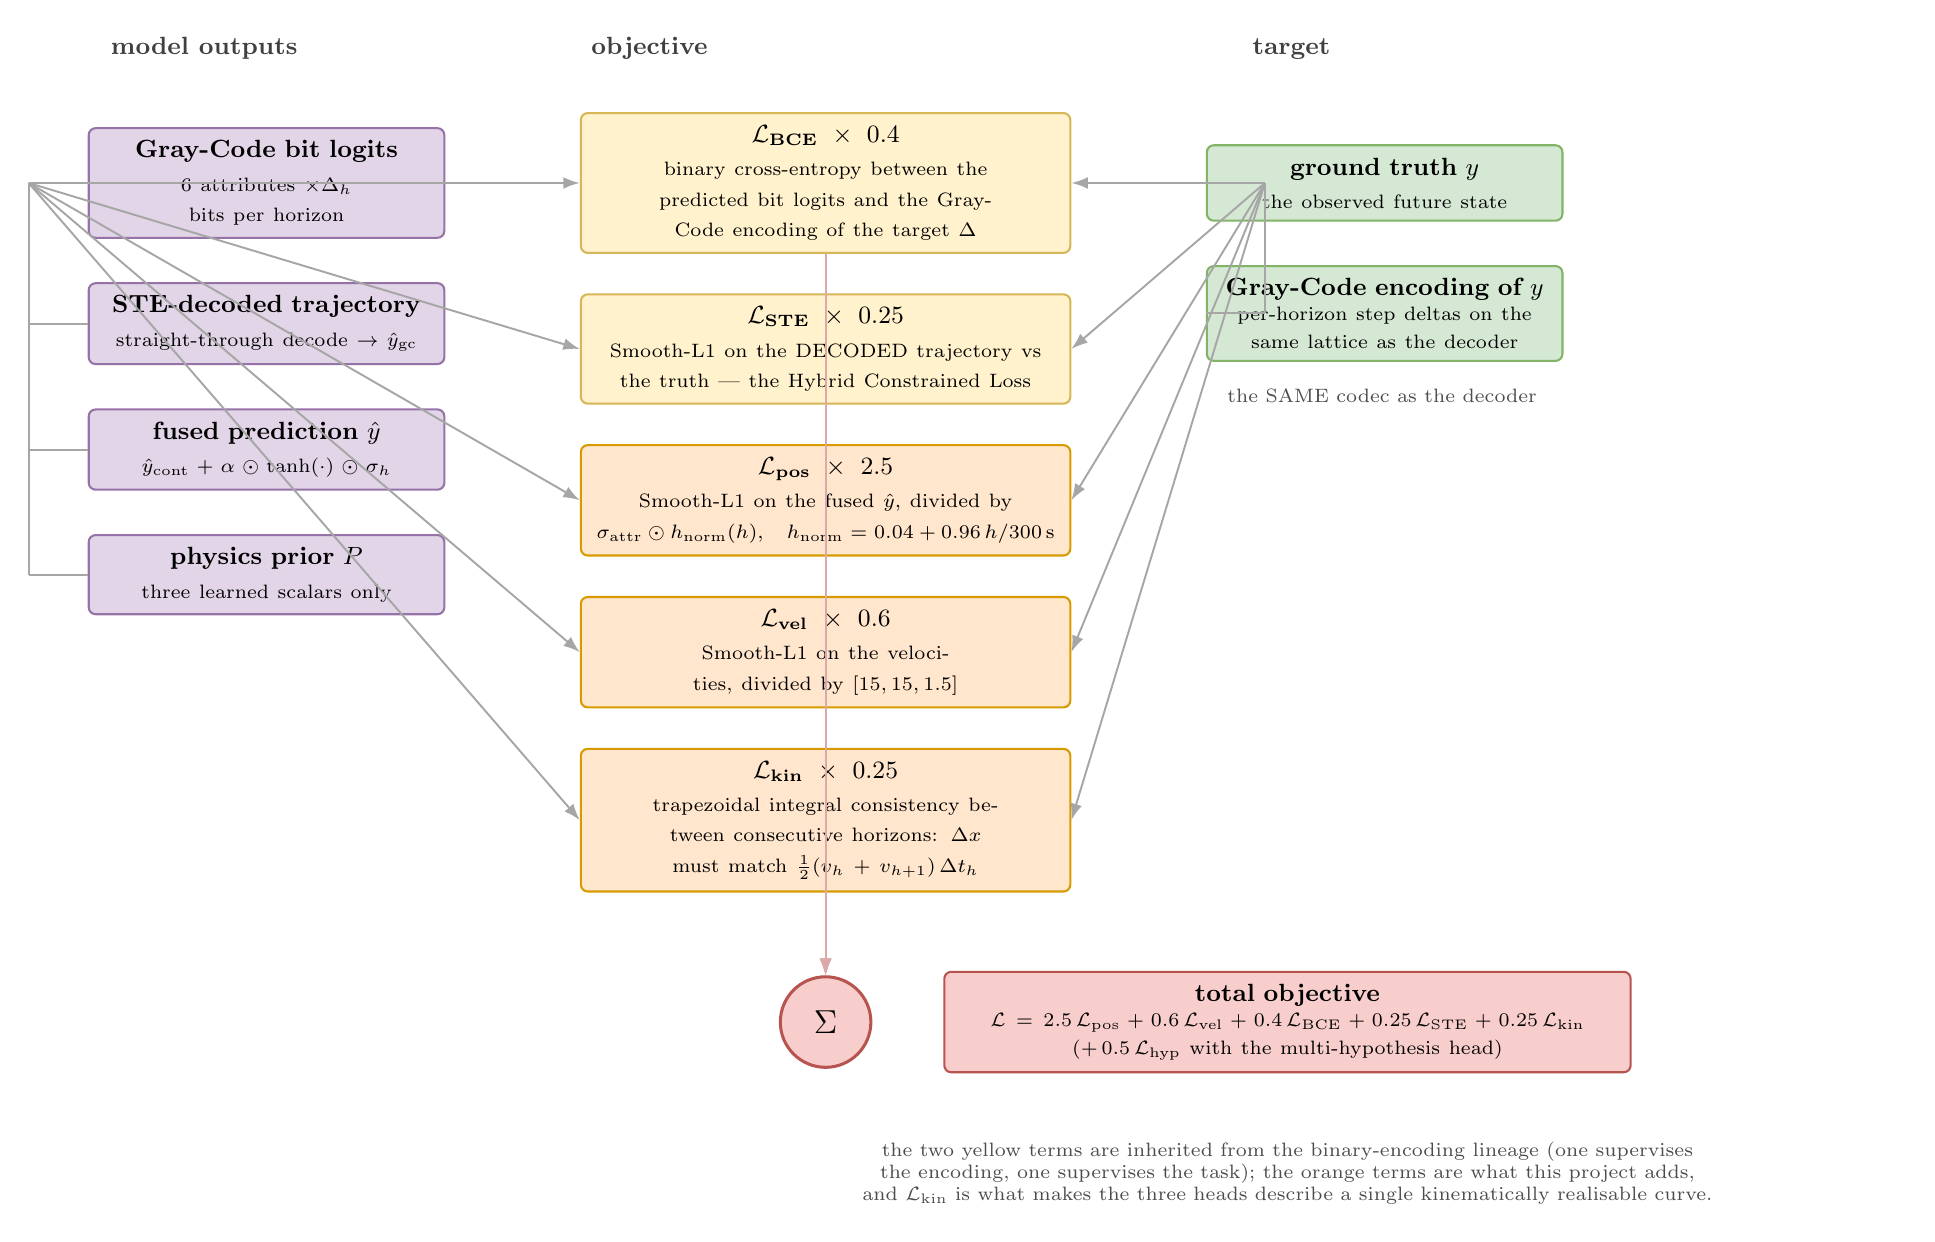
\begin{tikzpicture}

% ======================================================== model outputs (left)
\node[head, anchor=south west] at (-2.1,6.85) {model outputs};

\node[model] (logits) at (0,5.4)
  {\textbf{Gray-Code bit logits}\\[1pt]
   \scriptsize 6 attributes $\times \Delta_h$ bits per horizon};
\node[model, below=0.55cm of logits] (ygc)
  {\textbf{STE-decoded trajectory}\\[1pt]
   \scriptsize straight-through decode $\to \hat{y}_{\text{gc}}$};
\node[model, below=0.55cm of ygc] (yhat)
  {\textbf{fused prediction $\hat{y}$}\\[1pt]
   \scriptsize $\hat{y}_{\text{cont}} + \alpha \odot \tanh(\cdot) \odot \sigma_h$};
\node[model, below=0.55cm of yhat] (P)
  {\textbf{physics prior $P$}\\[1pt]
   \scriptsize three learned scalars only};

% ============================================================== target (right)
\node[head, anchor=south west] at (12.4,6.85) {target};
\node[tgt] (y) at (14.2,5.4)
  {\textbf{ground truth $y$}\\[1pt]
   \scriptsize the observed future state};
\node[tgt, below=0.55cm of y] (yenc)
  {\textbf{Gray-Code encoding of $y$}\\[1pt]
   \scriptsize per-horizon step deltas on the\\[-1pt]
   \scriptsize same lattice as the decoder};
\node[small, anchor=north west] at ($(yenc.south west)+(0.15,-0.22)$)
  {the SAME codec as the decoder};

% ================================================================ loss terms
\node[head, anchor=south west] at (4.0,6.85) {objective};

\node[inherited] (lbce) at (7.1,5.4)
  {\textbf{$\mathcal{L}_{\text{BCE}} \times 0.4$}\\[1pt]
   \scriptsize binary cross-entropy between the predicted bit logits
   and the Gray-Code encoding of the target $\Delta$};
\node[inherited, below=0.5cm of lbce] (lste)
  {\textbf{$\mathcal{L}_{\text{STE}} \times 0.25$}\\[1pt]
   \scriptsize Smooth-L1 on the DECODED trajectory vs the truth
   --- the Hybrid Constrained Loss};
\node[added, below=0.5cm of lste] (lpos)
  {\textbf{$\mathcal{L}_{\text{pos}} \times 2.5$}\\[1pt]
   \scriptsize Smooth-L1 on the fused $\hat{y}$, divided by
   $\sigma_{\text{attr}} \odot h_{\text{norm}}(h)$, \;
   $h_{\text{norm}} = 0.04 + 0.96\,h/300\,\text{s}$};
\node[added, below=0.5cm of lpos] (lvel)
  {\textbf{$\mathcal{L}_{\text{vel}} \times 0.6$}\\[1pt]
   \scriptsize Smooth-L1 on the velocities, divided by $[15, 15, 1.5]$};
\node[added, below=0.5cm of lvel] (lkin)
  {\textbf{$\mathcal{L}_{\text{kin}} \times 0.25$}\\[1pt]
   \scriptsize trapezoidal integral consistency between consecutive horizons:
   $\Delta x$ must match $\tfrac12(v_h + v_{h+1})\,\Delta t_h$};

% =================================================================== summation
\node[circle, draw=roleSumEdge, fill=roleSum, line width=1.1pt,
      inner sep=0pt, minimum size=1.15cm, font=\large\bfseries]
      (sum) [below=1.05cm of lkin] {$\Sigma$};
\node[total, right=0.9cm of sum] (tot)
  {\textbf{total objective}\\[1pt]
   \scriptsize $\mathcal{L} = 2.5\,\mathcal{L}_{\text{pos}} + 0.6\,\mathcal{L}_{\text{vel}}
   + 0.4\,\mathcal{L}_{\text{BCE}} + 0.25\,\mathcal{L}_{\text{STE}}
   + 0.25\,\mathcal{L}_{\text{kin}}$\\[-1pt]
   \scriptsize ($+\,0.5\,\mathcal{L}_{\text{hyp}}$ with the multi-hypothesis head)};

% ====================================================================== buses
% left bus (model outputs) and right bus (target)
\draw[bus] ($(logits.west)+(-0.75,0)$) -- ($(P.west)+(-0.75,0)$);
\draw[bus] ($(y.west)+(0.75,0)$) -- ($(yenc.west)+(0.75,0)$);
\draw[bus] (logits.west) -- ($(logits.west)+(-0.75,0)$);
\draw[bus] (ygc.west) -- ($(ygc.west)+(-0.75,0)$);
\draw[bus] (yhat.west) -- ($(yhat.west)+(-0.75,0)$);
\draw[bus] (P.west) -- ($(P.west)+(-0.75,0)$);
\draw[bus] (y.west) -- ($(y.west)+(0.75,0)$);
\draw[bus] (yenc.west) -- ($(yenc.west)+(0.75,0)$);
\foreach \n in {lbce,lste,lpos,lvel,lkin}{
  \draw[ar, draw=black!35] ($(logits.west)+(-0.75,0)$ |- \n.west) -- (\n.west);
  \draw[ar, draw=black!35] ($(y.west)+(0.75,0)$ |- \n.east) -- (\n.east);
}

% convergence into the summation node
\foreach \n in {lbce,lste,lpos,lvel,lkin}{
  \draw[ar, draw=roleSumEdge!50] (\n.south) -- ++(0,-0.16) -| (sum.north);
}

% ==================================================================== caption
\node[small, below=0.75cm of tot, text width=15.5cm, align=center]
  {the two yellow terms are inherited from the binary-encoding lineage (one supervises the
   encoding, one supervises the task); the orange terms are what this project adds, and
   $\mathcal{L}_{\text{kin}}$ is what makes the three heads describe a single kinematically
   realisable curve.};

\end{tikzpicture}
\end{document}
